%! Suppress = EnDash
\chapter[Setting Up]{Setting Up the Development Environment}\label{ch:setting-up}
\section{Introduction}\label{sec:setting-up-introduction}
To start developing software for the lab, you're going to need various different programs. The process of installing those programs will be different depending on your operating system. It's almost impossible to keep up-to-date, detailed sets of instructions for every possible version of each program, or for every possible hardware configuration. The steps below are generalized and should not present you with any issues. When in doubt, it's always best to either check the instructions that the package developers provide or ask in the forums.

\section{Choosing Pure Python or Anaconda}\label{sec:python-or-anaconda}
If you're already familiar with Python, then you probably know that there are different \textbf{distributions} that are worth discussing. In and of itself, Python is a text document that specifies what to expect when it encounters certain commands. This gives you much freedom to develop different implementations of those specifications, each one with different advantages. The \emph{official} distribution is available at python.org and is the distribution maintained by the Python Software Foundation. In the following sections, you'll see how to install it step by step. This distribution is also referred to as CPython because it's written in the programming language \textbf{C}. The official distribution follows Python's specifications to the letter. As a result, this is the one that comes bundled with Linux and Mac computers. Newer versions of Windows will start shipping the official Python distribution as well.

However, the base implementation of Python left room for improvement in certain areas. Some developers started to release optimized Python distributions that were tailored for specific tasks. For example, Intel released a specially-designed Python version to support multi-core architectures, one that leverages specific, low-level libraries that they developed themselves.

There are other versions of Python, such as Pypy, Jython, Iron Python, and others. Each one has its own merits and drawbacks. Some can run much faster in some contexts but at the expense of limiting the number of things that you can do. Between this wealth of options, there's one that's very popular amongst scientists and those doing numeric computations called \textbf{Anaconda}, which we cover in this book.

To expand Python, we can use external packages that can be developed and made publicly available. In the past, the Python package manager (pip) was limited; it allowed you to install only more straightforward packages. There was a clear need to have a tool that allowed the installation of more complex packages, including libraries not written in Python. Most numerical programs rely on libraries written in lower-level programming languages such as Fortran or C. Those libraries are not always easy to install on all operating systems, nor is it straightforward to keep track of their dependencies and versions. Anaconda was born to address these issues and is still thriving to this day.

Anaconda is a distribution of Python that comes with \emph{batteries included} for scientists. It includes many Python libraries by default as well as several supporting programs. It also contains a potent package manager that allows you to install highly-optimized libraries for different environments, regardless of whether you're using Windows, Linux, or Mac.

The first edition of this book included instructions for exclusively using pure Python because Anaconda is overkill for the purposes we're covering. However, it's common for researchers to have Anaconda installed on their computers. Therefore, we decided to show you how to work with it. If you're starting from scratch, we highly encourage you to begin with Anaconda, because it makes your life as a scientist much easier. However, if you're using a more limited computer or if your installation options are limited, then you can use pure Python. For this book, it's simple to install all the required libraries with either approach.

\section{Installing Anaconda}\label{sec:installing-anaconda}
To install Anaconda, you just need to head to the official website: anaconda.com. Go to the download section and select the installer for the newest version of Python. The site usually auto-detects your operating system and offers you either a graphical installation (recommended) or a command-line one. If you're on Linux, you have to be careful whether you want the Anaconda Python to become your default Python installation. Typically, there won't be any issues; you'll just need to be aware that other programs that rely on Python will use the Anaconda version and not the stock version.

\tipsInfo{Note}{Similar to the different distributions of Python, Anaconda also comes in two primary flavors: Anaconda and Miniconda. The main difference is that the latter bundles fewer programs and is therefore lighter to download. Unless you're very low in space on your computer or have particular requirements, we strongly recommend downloading the full installation for Anaconda.}

\subsection{Using Anaconda}\label{subsec:using-anaconda}
Even though Anaconda comes with a graphical interface to install packages, it's highly recommended that you use the command line because it's easier to transmit ideas with words. If you're on Windows, you need to start a program called \emph{Anaconda Prompt}, as shown in the image below:

\begin{center}
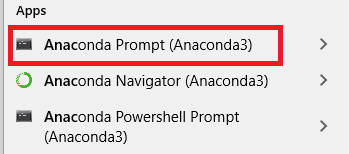
\includegraphics[width=.5\textwidth]{images/Chapter_02/AnacondaPrompt_Menu.png}
\end{center}

If you're on Linux, you only need to open a terminal. On Ubuntu, you can do this by pressing Ctrl+Alt+T. What's important to note is that when you trigger Anaconda, you'll see that your command line has a \mintinline{bash}{(base)} prepending it, as shown in the image below:

\begin{center}
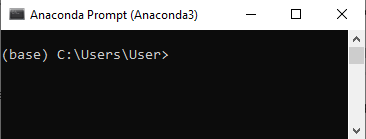
\includegraphics[width=.5\textwidth]{images/Chapter_02/AnacondaPrompt.png}
\end{center}

This is the best indication to know you're running the Anaconda installation.

You can run the following command to see all the installed packages:

\begin{minted}{bash}
conda list
\end{minted}

The output you'll see will depend on what you have installed and whether or not you've already used Anaconda in the past. You'll see that at the beginning it tells you where your Anaconda installation is, followed by four columns: Name, Version, Build, and Channel. It should look something like this:

\begin{minted}{bash}
# packages in environment at /opt/anaconda3:
#
# Name                    Version                   Build  Channel
matplotlib                3.1.3                    py37_0
numpy                     1.18.1           py37h4f9e942_0
pyyaml                    5.3              py37h7b6447c_0
yaml                      0.1.7                had09818_2
\end{minted}

This image shows a few example packages, but your output should be much longer.

One of the good things about Anaconda is that it keeps track of each package, its version, and the build. The difference is that you may be using Anaconda on a computer with an Intel processor, or a Raspberry Pi with an ARM processor. In both cases, the version of, let's say, \py{numpy} may be the same, but they were compiled differently. You could also be using the same version of \py{numpy} but with a different version of Python (hence the \py{py37} that appears in the build numbers) which allows you to keep track of what you're doing at any given moment.

The last two lines show you a package called \py{pyyaml} that depends on a library called \py{yaml}, which you'll use later. With Anaconda, you can separately keep track of both the Python package and the lower-level library that this package uses. If you're coming from Linux, this won't be a great surprise, since this is precisely what the package manager on your computer does. If you're coming from Windows, however, this is something incredibly handy.

Say you want to install a package that you don't yet have on your machine. Let's see how you would install \py{PySerial}, which is a package that you'll use later in the book. Installing it becomes as easy as running the following command:

\begin{minted}{bash}
conda install pyserial
\end{minted}

This command outputs some information, such as the version and the build, then asks if you want to install it. You can select 'yes' and it will proceed. If you list the installed packages again, you'll notice that PySerial is listed there.

But this is not all Anaconda allows you to do. You can also use separate environments based on your projects.

\subsection{working with conda environments}\label{subsec:conda-environments}
A \textbf{conda environment} is, in practical matters, a folder where all the packages that you'll need to run your code are located, including any underlying libraries. the environments are \textbf{isolated} from each other; in other words, updating or deleting a package in one environment won't affect the state of that same package in any other environment. when you're working on different projects, there may be times where one needs a specific library version, and you don't want to ruin the other projects. to create a new environment, you need to run the following command (changing \py{myenv} to any name you want):

\begin{minted}{bash}
 conda create --name myenv
\end{minted}

then you activate it:

\begin{minted}{bash}
 conda activate myenv
\end{minted}

now if you list the installed packages you'll see there's nothing there:

\begin{minted}{bash}
conda list
# packages in environment at /opt/anaconda3/envs/myenv:
#
# name                    version                   build  channel
\end{minted}

from here, in your newly created environment, it's time to install the packages you want, starting with python itself:

\begin{minted}{bash}
 conda install python=3.7
\end{minted}

this will install the specified version of python in your new environment.

\infoInfo{Python Versions}{The \py{3.7} that you added after \py{python=} specifies which version of Python we want to use. If you don't specify it, then Anaconda installs the latest version, which at the time of writing is \py{3.8}. When Python updates, some libraries may not work correctly, or they  may not yet be available for that specific version. When selecting the Python version, be sure all your libraries are available.}

After installing Python, you can run it by typing:

\begin{minted}{bash}
 python
\end{minted}

The output will look something like this:

\begin{minted}{text}
Python 3.7.7 (default, Mar 26 2020, 15:48:22)
[GCC 7.3.0] :: Anaconda, Inc. on linux
Type "help", "copyright", "credits" or "license" for more information.
\end{minted}

To exit, just type:

\begin{minted}{bash}
exit()
\end{minted}

To follow the book, you'll need these packages:

\begin{itemize}
 \item NumPy -> For working with numerical arrays
 \item pySerial -> For communicating with serial devices
 \item PyYAML -> For working with YAML files, a specially structured text file
 \item PyQt -> For building Graphical User Interfaces
 \item PyQtGraph -> For plotting results within the User Interfaces
\end{itemize}

You can install all of these by running:

\begin{minted}{bash}
conda install numpy pyserial pyyaml pyqt pyqtgraph
\end{minted}

Don't worry too much about these packages, since you'll see them one-by-one later on.

If you run \mintinline{bash}{conda list}, you'll see that there are \emph{many} more packages installed. Each package depends either on other packages or libraries, and Anaconda took care of installing all of them for you. With a \mintinline{bash}{conda install} command, you can install packages that Anaconda itself maintains. These are official packages that come with a certification of quality. Many companies will allow their employees to only install packages that are officially supported by Anaconda, in order to avoid having malware installed within their network.

To follow the book, you'll need one more package called \py{Pint}. This package is \emph{not} in the official conda repositories. To install packages that aren't yet in the official repository, you can use an unofficial repository called \py{conda forge}. Packages that aren't mature enough, or versions that are too new and not tested enough, are located in this repository. To install a package, you just need to run the following command:

\begin{minted}{bash}
  conda install -c conda-forge pint
\end{minted}

The \mintinline{bash}{-c conda-forge} specifies the \py{channel} you want to install the package from. With this, you've finished installing all the packages you'll need to follow the rest of the book.

If you want to leave the environment, you can run:

\begin{minted}{bash}
conda deactivate
\end{minted}

This should return you to your normal shell prompt.

\subsubsection{Creating environments more quickly}
In the steps above, you created an empty environment and then installed the necessary packages. You can perform this operation slightly faster if you already know what you need. For example, you can do the following:

\begin{minted}{bash}
conda create --name env python=3.7 numpy=1.18 pyserial
\end{minted}

The command above creates an environment using the specified versions of Python and NumPy while using the latest version of PySerial.

\subsubsection{Removing an environment}
If you want to remove a conda environment called \py{env}, you can run the following command:

\begin{minted}{bash}
conda remove --name env --all
\end{minted}

\sloppy In practice, you also use the \py{remove} command to uninstall packages. When you do \py{remove --name env} it means that you want to remove a specific package from that environment, while the \py{--all} option tells Anaconda to remove \emph{all} the packages \emph{and} the environment itself. Use with care, since you can't undo it!

\section{Installing Pure Python}\label{sec:installing-pure-python}
If instead of Anaconda you prefer to install pure Python, the procedure is quite straightforward. It just varies slightly on different operating systems.

\subsection{Installing Python on Windows}\label{subsec:python-installation-on-windows}
Windows doesn't come with a pre-installed version of Python, so you'll need to install it yourself. Fortunately, it's not a complicated process. Go to the download page at Python.org, where you'll find a link to download the latest version of Python.

\tipsInfo{Note}{We've tested all the contents of this book with Python 3.7, but newer versions shouldn't give you any problems. If you install a more recent version and run into any problems later on, come back to this step, uninstall Python, and then reinstall an older version.}

Once the download is complete, you should launch the installer and follow the steps to install Python on your computer. Be sure that you select \textbf{Add Python 3.7 to the PATH}. If there are more users on the computer, you can also select \emph{Install Launcher} for all users. Just click on \textit{Install Now} and you're good to go! Pay attention to the messages that appear, just in case anything goes wrong.

\subsubsection{Testing your installation}
To test whether your installation of Python is working, you need to launch the Command Prompt, which is the Windows equivalent to a Terminal in most Unix operating systems. Throughout this book, we'll use the terms Command Prompt, Command Line, or Terminal interchangeably.

The Command Prompt is a program that allows you to interact with your computer by typing commands instead of using the mouse. To launch it, click the Start Button and search for \emph{Command Prompt} (it may be located in the Windows System apps). It should look like the image you see below:

\begin{center}
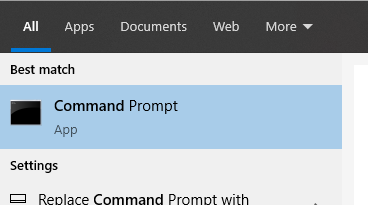
\includegraphics[width=.5\textwidth]{images/Chapter_02/CommandPrompt.png}
\end{center}

In the Command Prompt, you can do almost everything that you can do with the mouse on your computer. The command prompt starts in a specific folder on your computer, something similar to \mintinline{PowerShell}{C:\Users\User}. You can type \mintinline{bash}{dir} and press enter to get a list of all the files and folders within that directory. If you want to navigate through your computer, you can use the command \mintinline{bash}{cd}, which stands for \emph{change directory}. If you want to go one level up, then you can type \mintinline{bash}{cd ..}, where the two dots \mintinline{bash}{..} represent the parent folder of the one you're currently located in. If you want to enter a folder, then you type \mintinline{bash}{cd Folder} where \textit{Folder} is the name of the folder you want to change to.

It's out of the scope of this book to cover all the different possibilities that the Command Prompt offers you, but you shouldn't have any problems finding help online. See the image below to get an idea of what using the Command Prompt looks like on Windows:

\begin{center}
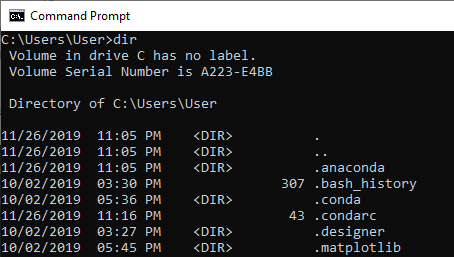
\includegraphics[width=.5\textwidth]{images/Chapter_02/CommandPrompt03.png}
\end{center}

To test that your Python installation was successful, just type \mintinline{bash}{python.exe} and hit enter. You should see a message like this:

\begin{minted}{powershell}
Python 3.7.7 (default, Oct  3 2017, 21:45:48)
[GCC 7.2.0] on Win64
Type "help", "copyright", "credits" or "license" for more information.
\end{minted}

The output shows you which Python version you're using as well as some extra information. You've just started what's called the Python Interpreter, which is an interactive way of using Python. If you come from a Matlab background, then you'll notice its similarities immediately. Go ahead and try it with some mathematical operation, like adding or dividing numbers:

\begin{minted}{pycon}
>>> 2+3
5
>>> 2/3
0.6666666666666666
\end{minted}

For future reference, when you see lines that start with \mintinline{pycon}{>>>} it means that you're working within the Python Interpreter. The lines without \mintinline{pycon}{>>>} in front are the output generated by the program.

\subsection{Adding Python to the PATH on Windows}\label{subsec:path-windows}
If you receive an error message saying that the command \mintinline{bash}{python.exe} was not found, then something went slightly wrong with the installation. Remember when you selected \textbf{Add Python to the PATH}? That option is what tells the Command Prompt where to find the program \mintinline{bash}{python.exe}. If, for some reason, it didn't work while installing, then you'll have to do this manually.

First, you need to find out where your Python is installed. If you paid attention during the installation process, then that shouldn't be a problem. Most likely you can find it in a directory like this one:

\begin{minted}{powershell}
C:\Users\**YOURUSER**\AppData\Local\Programs\Python\Python36
\end{minted}

Once you find the file \mintinline{bash}{python.exe}, copy the full path of that directory (that is, the location of the folder where you found \mintinline{bash}{python.exe}). You then have to add that file location to the system variable called PATH. Here are the steps you'll need to take:

\begin{enumerate}
    \item Open the System Control Panel. How to open it is slightly dependent on your Windows version, but it should be something like \emph{Start/Settings/Control Panel/System}.
    \item Open the \emph{Advanced} tab.
    \item Click the \emph{Environment Variables} button.
    \item Find the section called \emph{System Variables}. Select \emph{Path}, then click \emph{Edit}. You'll see a list of folders, each one separated from the next one by a semicolon (\py{;}).
    \item Add the folder where you found the \mintinline{bash}{python.exe} file at the end of the list. Don't forget the semicolon (\py{;}) to separate it from the previous entry.
    \item Click OK\@.
\end{enumerate}

You'll have to restart the Command Prompt for it to refresh the settings. Try to run \mintinline{bash}{python.exe} again and it should work.

\subsection{Installing Python on Linux}\label{subsec:installation-on-linux}
Most Linux distributions come with Python already installed. To check whether it's already on your system, open up a terminal (Ubuntu users can press Ctrl+Alt+T). You can then type \mintinline{bash}{python3}, and press enter. If it works you should see something like this appear on the screen:

\begin{minted}{bash}
Python 3.6.3 (default, Oct  3 2017, 21:45:48)
[GCC 7.2.0] on Linux
Type "help", "copyright", "credits" or "license" for more information.
\end{minted}

If it doesn't work, then you need to install Python 3 on your system. Ubuntu users can do this by running the following:
\begin{minted}{bash}
sudo apt install python3
\end{minted}

Each Linux distribution has a slightly different way of installing Python, but all of them more or less follow the same procedure. After the installation, check to see if it went well by typing \mintinline{bash}{python3} and hitting enter. Future releases of the operating system will include only Python 3 by default, and you won't need to add the \emph{3} explicitly. In case there's an error, try running only \mintinline{bash}{python} first and check whether your machine recognizes that you want to use Python 3.

\subsection{Installing Python packages}\label{subsec:installing-python-packages2}\label{subsec:installing-python-packages}
One of the characteristics that makes Python such a versatile programming language is the variety of packages that you can use in addition to the standard library. Python has a repository of applications called PyPI, which stands for the Python Package Index. PyPI contains more than one hundred thousand packages. The easiest way to install and manage these packages is through a command called \textbf{pip}. pip fetches the needed packages from the repository and installs them for you. pip is also capable of removing and upgrading packages. More importantly, pip handles dependencies so you don't have to worry about them.

pip works both with Python 3 and Python 2. To avoid mistakes, you have to be sure that you're using the version of pip that corresponds to the Python version you want to use. If you're on Linux and have both Python 2 and Python 3 installed, there are probably two commands, \py{pip2} and \py{pip3}. You should use the latter to install packages for Python 3. On Windows, you likely have to use \mintinline{PowerShell}{pip.exe} instead of just \mintinline{bash}{pip}. If this doesn't work for some reason, you'll need to follow the same procedure that you saw earlier to add \mintinline{bash}{python.exe} to the PATH, but this time with the location of your \mintinline{bash}{pip.exe} file.

\tipsInfo{Info}{Since the moment Anaconda was born up until now, pip has gone through many trials and tribulations. Today, you can install complex packages such as NumPy or PyQt directly. However, there's still some discussion regarding how much we can expect from pip at the moment as far as compiling programs or performing complex tasks.}

Now, installing a package becomes very simple. If you'd like to install a package such as NumPy, you should just type the following:
\begin{minted}{bash}
pip install numpy
\end{minted}

Windows users should type this:
\begin{minted}{powershell}
pip.exe install numpy
\end{minted}

\warningInfo{Before You Continue}{Before installing the packages listed below, it's essential that you read the following section on \textbf{Virtual Environments}. These will help you maintain clean and separate environments for software development.}

\begin{itemize}
 \item NumPy -> To work with numerical arrays
 \item Pint -> To use units and not just numbers
 \item pySerial -> To communicate with serial devices
 \item PyYAML -> To work with YAML files, a specially structured text file
 \item PyQt5 -> To build Graphical User Interfaces
 \item PyQtGraph -> To plot results within the User Interfaces
\end{itemize}

\sloppy You can install all the packages with pip without trouble. If you're in doubt, you can search for packages by typing \mintinline{bash}{pip search package_name}. Usually, the order in which you install the packages doesn't matter. Notice that since pip installs the dependencies, you sometimes get a message saying that a package is already installed, even if you didn't do it manually.

To build user interfaces, we've decided to use Qt Designer, an external program provided by the creators of Qt. You don't need to have this program installed to develop a graphical application because you can do everything directly from within Python itself. However, this approach can be much more time-consuming than dragging and dropping elements onto a window.

\subsection{Working with virtual environments}\label{subsec:virtual-environment2}
When you start developing software, it is of the utmost importance that you have an \textbf{isolated programming environment} to precisely control the packages that are installed. For example, you can use experimental libraries without overwriting software that other programs use on your computer. With virtual environments, you can update a package within that specific environment only, without altering the dependencies for any additional development you might be doing.

If you're working in a lab, then it's even more critical to isolate different environments. In essence, you're developing a program with a specific set of libraries, each with its own version and installation method. One day you or another researcher who works with the same setup might decide to try out a program that requires slightly different versions for some of the packages. The outcome can be a disaster: If there's an incompatibility between the new libraries and the computer software, then you could ruin the very program that controls your experiment!

Unintentional library upgrades can set you back several days. Sometimes it might be so long since you installed a library that you can no longer remember how to do it or where to get the same version you had. Other times you may want to check what would happen if you were to upgrade a library, or you might wish to reproduce the set of packages installed by a different user to troubleshoot any issues. There's no way of overestimating the benefits of isolating environments on your computer.

Fortunately, Python provides you with \textbf{virtual environments} that give you a lot of control and flexibility. A virtual environment is nothing more than a folder where you'll find copies of the Python executable and all the packages you installed. Once you activate the virtual environment, every time you trigger pip for installing a package, it will do so within that directory. The Python interpreter will be the one inside the virtual environment and not any other one. It may sound complicated, but in practice, it's incredibly simple.

You can create isolated working environments for developing software to run specific programs or for performing tests. If you need to update or downgrade a library, you'll do so within that specific virtual environment, and you won't alter the functioning of anything else on your computer. It may take some time for you to acknowledge the advantages of using virtual environments, but once you lose days or even weeks reinstalling packages because something went wrong and your experiment doesn't run anymore, you'll understand.

\criticalInfo{Warning}{Virtual environments are excellent for isolating Python packages, but many packages rely on libraries installed on the operating system itself. If you need a higher degree of isolation and reproducibility, you should check out Anaconda.}

\subsubsection{Working with virtual environments on Windows}
Windows doesn't have the most user-friendly command line, and some of the tools you can use for Python are slightly trickier to install than on Linux or Mac. The steps below will guide you through the installation and configuration of virtual environments on a Windows machine. If something is failing, then try to find help or examples online. There are a lot of great examples on StackOverflow, for instance.

Python comes bundled with a tool for creating virtual environments, so you can install the package with pip:

\begin{minted}{powershell}
pip.exe install virtualenv
pip.exe install virtualenvwrapper-win
\end{minted}

To create a new environment called \mintinline{bash}{Testing} you have to run the following:

\begin{minted}{powershell}
mkvirtualenv Testing --python=path\to\python\python.exe
\end{minted}

The last piece is crucial because it allows you to select the exact version of Python you want to run. If you have more than one version of Python installed, then you can choose whether you wish to use, for instance, Python 2 or Python 3 for that specific project. The command also creates a folder called Testing, where you'll find all the required packages and programs. If everything went well, then you should see that your command prompt now displays a \mintinline{bash}{(Testing)} message before the path. This means that you are indeed working inside the environment.

Once you've finished working on your project and you want to leave the virtual environment, you can type the following:

\begin{minted}{powershell}
deactivate
\end{minted}

This will return you to the normal command prompt. If you want to work on \mintinline{bash}{Testing} again, you have to type:

\begin{minted}{powershell}
workon Testing
\end{minted}

If you want to test that things are working fine, you can upgrade pip by running:

\begin{minted}{powershell}
pip install --upgrade pip
\end{minted}

If there's a new version available, then it will be installed. One of the most useful commands to run within a virtual environment is this:

\begin{minted}{powershell}
pip freeze
\end{minted}

This command gives you a list of all the packages installed within that working environment and their exact versions. This is so you'll know what you're using and can revert if anything goes wrong. Moreover, for people who are worried about the reproducibility of the results, keeping track of specific packages is a great way to be sure that you can repeat everything later.

You can install the packages listed before, such as NumPy and PyQt5, and see that they will only be installed within your \mintinline{bash}{Testing} environment. If you activate or deactivate the virtual environment, the packages you installed within it will not be available, which you can see with \mintinline{bash}{pip freeze}.

\subsubsection{Working with virtual environments in Windows PowerShell}
If you're using Windows PowerShell instead of the Command Prompt, there are some things that you have to change. First is the virtual environment wrapper package, which needs to be installed separately for PowerShell:

\begin{minted}{powershell}
pip install virtualenvwrapper-powershell
\end{minted}

Most likely, you'll need to change the execution policy of scripts on Windows. Open a PowerShell with administrative rights (to do so, right-click on the PowerShell icon and then select \emph{Run as Administrator}). Then run the following command:

\begin{minted}{powershell}
Set-ExecutionPolicy RemoteSigned
\end{minted}

Follow the instructions that appear on the screen to allow the changes on your computer. This should allow the wrapper to work. You can repeat the same commands that you saw before to create a virtual environment.

If it still doesn't work, don't worry too much. Sometimes there's a problem with the wrapper, but you can still create a virtual environment by running the following:

\begin{minted}{powershell}
virtualenv.exe Testing --python=path\to\python\python.exe
\end{minted}

This command creates the virtual environment within the Testing folder. Go to the folder Testing/Scripts and run:
\begin{minted}{powershell}
.\activate
\end{minted}

Now you're running within a virtual environment in PowerShell.

\subsubsection{Working with virtual environments on Linux}
Installing the virtual environment packages on Linux is more routine. Depending on where you installed Python, you may need root access to follow the installation. If you're unsure, first try to run the commands without \mintinline{bash}{sudo}, and if they fail, run them with \mintinline{bash}{sudo} as shown below:

\begin{minted}{bash}
sudo -H pip3 install virtualenv
sudo -H pip3 install virtualenvwrapper
\end{minted}

If you're on Ubuntu, you can install the package through apt, although it's not recommended:
\begin{minted}{bash}
sudo apt install python3-virtualenv
\end{minted}

To create a virtual environment, you need to know where to find the Python version you would like to use. The easiest way to do this is to note the output of the following command:

\begin{minted}{bash}
which python3
\end{minted}

The output will tell you the location of the program that's triggered when you run \mintinline{bash}{python3} in a terminal. Replace the location of Python in the following command:
\begin{minted}{bash}
mkvirtualenv Testing --python=/location/of/python3
\end{minted}

This creates a folder, usually \mintinline{bash}{~/.virtualenvs/Testing}, with a copy of the Python interpreter and all the packages that you need, including pip. That folder is your virtual environment and is the place where new modules will be installed. If everything went well, then you'll see the \mintinline{bash}{(Testing)} string at the beginning of the line in your terminal. When you see it, you know that you're working within a virtual environment.

To close the virtual environment you have to type the following:

\begin{minted}{bash}
deactivate
\end{minted}

To work in the virtual environment again, just do this:
\begin{minted}{bash}
workon Testing
\end{minted}

If for some reason the wrapper isn't working, you can create a virtual environment manually by executing the following code:
\begin{minted}{bash}
virtualenv Testing --python=/path/to/python3
\end{minted}
Then, you can activate it by executing the following command:
\begin{minted}{bash}
source Testing/bin/activate
\end{minted}

Bear in mind that in this way, you create the virtual environment wherever you are on your computer and not in the default folder. This behavior can be handy if, for example, you want to share the virtual environment with somebody, or place it in a precise location on your computer.

Once you've activated the virtual environment, you can install the packages listed before, such as NumPy. You can compare what happens when you're in the environment to what happens outside, and check that you truly are isolated from the central Python installation. The packages that you install inside of \mintinline{bash}{Testing} should not be available outside of it.

One of the most useful commands to run within a virtual environment is this:

\begin{minted}{bash}
pip freeze
\end{minted}

This command gives you a list of all the packages installed within that working environment and their exact versions. This is so you'll know what you're using and can revert the package version if anything goes wrong. Moreover, for people who are worried about the reproducibility of the results, keeping track of specific packages is a great way to be sure that anyone can repeat the results at a later time.

\section{Using Qt Designer}\label{sec:install-qt-designer}
Qt Designer is a great tool to quickly build user interfaces by dragging and dropping elements onto a canvas. It allows you to swiftly develop elaborate windows and dialogs, styling them and defining some basic features without writing actual code. We use this program to design a detailed window in which the user can tune the experiment parameters and display data in real-time.

If you're using \textbf{Anaconda}, the Designer comes already bundled with it, so you don't need to follow the steps below.

\subsection{Installing Qt Designer on Windows}\label{subsec:installing-on-windows}
Installing Qt Designer on Windows only takes one Python package: \mintinline{bash}{pyqt5-tools}. Run the following command:

\begin{minted}{bash}
pip install pyqt5-tools
\end{minted}

\sloppy The designer should be located in a folder called \mintinline{bash}{pyqt5-tools}. The folder's location depends on how you installed Python and whether you're using a virtual environment. If you aren't sure, then use the tool to find folders and files in your computer and search for \mintinline{bash}{designer.exe}.

\tipsInfo{Info}{The package \mintinline{bash}{pyqt5-tools} is an independent package aimed at making the installation of the Qt Designer easier. However, it takes a bit of time for it to update to the latest version of Python. At the time of this writing, it's known to work with Python 3.7, but not with Python 3.8.}

\subsection{Installing Qt Designer on Linux}\label{subsec:installing-on-linux}
Linux users can install Qt Designer directly from within the terminal by running the following command:

\begin{minted}{bash}
sudo apt install qttools5-dev-tools
\end{minted}

To start the Designer, just look for it within your installed programs, or type \mintinline{bash}{designer} and press enter in a terminal.

\section{Choosing a Text Editor}\label{sec:editors}
To complete the Python For The Lab book, you'll need a \textbf{text editor}. As with many decisions in this book, you are entirely free to choose whichever one you like. Still, there are some resources we'll point out that can be useful to you.

You won't need anything more sophisticated for editing code than a \textbf{plaintext editor}, such as Notepad++. This is available on Windows only, and it's very basic and straightforward. You can have several tabs open with different files and you can perform a search for a specific string in your opened documents, or even within an entire folder. Notepad++ is very good for small changes to code, perhaps made directly in the lab. The equivalent to Notepad++ on Linux are text editors such as Gedit or Kate. Every Linux distribution comes with a pre-installed text editor.

Developing software for the lab requires working with different files simultaneously, being able to check that your code is correct before running it, and ideally being able to interface directly with virtual environments (whether you're using conda or virtualenv). For all this, there is a range of programs called IDEs or \textbf{Integrated Development Environments}. We strongly suggest you check out \textbf{PyCharm}, which offers a free and open-source Community Edition as well as a Professional Edition (which you can get for free if you're a student or teacher affiliated with a university). PyCharm integrates itself with virtual environments and allows you to install a package if it's missing, but you need it and many more things. It's a sophisticated program, but there are many great tutorials on how to get started. Familiarizing yourself with PyCharm pays off quickly.

Another very powerful IDE for Python is \textbf{Microsoft's Visual Studio Code}, which is very similar to PyCharm in it's capabilities. If you have previous experience with Visual Studio, I strongly suggest you keep using it. It integrates very nicely with your workflow. Visual Studio is available not only for Windows but also for Linux and Mac. It has some excellent features for inspecting elements and helping you debug your code. The community edition is free of charge. Support for Python is complete, and Microsoft has released several video tutorials showing you how to get the best out of their program.

There are other options around, such as Atom or Sublime. However, they don't specifically target Python as the previous two do. Remember that the choice is always yours. Editors should be a tool and not an obstacle. If you've never used an IDE before, then we recommend you just go ahead and install PyCharm. That's what we use during the workshops, and everyone has always been very pleased with it. If you already have an IDE or a workflow with which you are happy, then keep it! If at some point it starts failing you, then you can reevaluate the situation.

\warningInfo{Tabs or Spaces}{Python is sensitive to the use of \textbf{tabs} and \textbf{spaces}. You shouldn't mix them! A good standard is to use four spaces to indent your code. If you decide to go for a text editor, then be sure to configure it to respect Python's stylistic choices. Notably, Notepad++ comes preset to use tabs instead of spaces, which is a problem if you ever copy and paste code from other sources.}
